\documentclass[10pt,twocolumn]{article}

\usepackage[a4paper,margin=0.68in,columnsep=0.23in]{geometry}
\usepackage{graphicx}
\usepackage{booktabs}
\usepackage{amsmath}
\usepackage{microtype}
\usepackage{enumitem}
\usepackage{caption}
\usepackage[hidelinks]{hyperref}
\usepackage{xcolor}
\usepackage{placeins}

\captionsetup{font=small,labelfont=bf}
\setlength{\parindent}{1em}
\setlength{\parskip}{0.12em}
\setlist[itemize]{leftmargin=1.3em,itemsep=0.05em,topsep=0.15em}
\newcommand{\pc}{\textnormal{\textsc{ProbCover}}}
\newcommand{\mh}{\textnormal{\textsc{MaxHerding}}}
\newcommand{\tc}{\textnormal{\textsc{TypiClust}}}
\newcommand{\npc}{\textnormal{\textsc{NPC}}}
\newcommand{\ce}{\textnormal{\textsc{CE}}}
\newcommand{\gce}{\textnormal{\textsc{GCE}}}
\newcommand{\dataset}{\textnormal{\textsc{CIFAR-100}}}
\newcommand{\RawRuns}{456}
\newcommand{\DuplicateRuns}{8}
\newcommand{\UniqueRuns}{448}
\newcommand{\RunsPerBudget}{224}
\newcommand{\PCSymKNNDelta}{+2.90}
\newcommand{\PCSymCVDelta}{+2.30}
\newcommand{\PCSymAUMDelta}{+1.05}
\newcommand{\MHSymLead}{1.54}
\newcommand{\PCAsymLead}{1.56}
\newcommand{\GCEFourDelta}{-10.83}
\newcommand{\GCEEightDelta}{-6.90}


\title{Active Learning with Noisy Labels at a Small Budget\\
\large What Worked, What Failed, and What I Learned from 448 Runs}
\author{Tom Novak}
\date{Master's project report -- August 2026}

\begin{document}
\maketitle
\vspace{-1.0em}

\begin{abstract}
This project studies active learning (AL) under label noise and a limited
annotation budget. I evaluated six standard selection methods, four
direct label-cleaning methods, three robust losses, and noise-aware versions of
\pc{} and \mh{} on frozen self-supervised features from \dataset{}. The final
CSV contains \RawRuns{} completed rows. Eight rows are duplicate ordinary
\mh{} baselines, leaving \UniqueRuns{} unique configurations. The main metric
is 1-nearest-neighbor (1-NN) test accuracy, because it measures the quality of
the selected labeled set directly. Losses are compared with a trained linear
classifier. Coverage-based methods are the strongest standard selectors. Direct
cleaning has almost no effect on the linear classifier, and \gce{} is much
worse than cross-entropy. Noise-aware \pc{} becomes useful at 800 labels,
especially under symmetric noise, but the same practical detectors usually
hurt \mh{}. Overall, noise-aware selection appears promising, but its success
depends strongly on the selector, the noise type, and the amount of labeled
data available to the detector.
\end{abstract}

\section{Motivation and setup}

In pool-based AL, the learner repeatedly chooses which unlabeled images should
be annotated next. The aim is to reach good accuracy with fewer labels.
This becomes harder when the annotator is noisy: a selected image may receive
the wrong class, so a well-chosen image can still provide misleading
supervision. My project separates three questions: which images should be
selected, whether suspicious labels should be changed, and whether the
classifier should use a noise-robust loss.

All experiments use \dataset{} and fixed 512-dimensional self-supervised
features. The labeled set starts with 100 images and each AL round adds 100.
The two final budgets are 400 and 800 labels, corresponding to three and seven
query rounds. Synthetic symmetric and asymmetric noise use a rate of 0.5. I
also include clean labels and CIFAR-100N human annotations
\cite{wei2022cifarn}. Every configuration uses seed 42. After deduplication
there are \RunsPerBudget{} runs at each budget.

The main evaluation is 1-NN on the test set using the final labeled examples as
the reference set. This metric depends on both the chosen images and their
stored labels. I also train a single linear layer on the frozen features. It is
important to call this model a \emph{linear classifier}, not an MLP: the code
contains optional hidden layers, but they are disabled in these runs. The
linear score is the correct metric for comparing training losses.

\section{Methods in the comparison}

\subsection{Standard AL selectors}

\textbf{Random} samples uniformly and serves as the basic reference. \textbf{Margin}
selects images for which the classifier's two largest probabilities are close.
It can be unreliable early on, when there are only one or two labeled
examples per class. \textbf{CoreSet} uses greedy $k$-center selection and tries
to reduce the largest distance from the unlabeled pool to the labeled set
\cite{sener2018coreset}. \textbf{\tc{}} clusters the features and prefers
typical points from dense regions \cite{hacohen2022typiclust}.

\textbf{\pc{}} treats a point as covered when it lies within a fixed radius
$\delta$ of a labeled example. It greedily selects points that cover many new
neighbors \cite{yehuda2022probcover}. \textbf{\mh{}} uses the same coverage
idea with a smooth RBF kernel instead of a hard radius. A nearby point receives
partial coverage rather than an all-or-nothing decision
\cite{bae2024maxherding}. Both methods use normalized frozen features.

\subsection{Direct label handling}

The direct methods are applied after training each AL episode. \textbf{Checkpoint
cleaning} replaces a label when the classifier predicts another class with
confidence at least 0.7. \textbf{Cross-validation cleaning} uses five folds so
that a sample is predicted by a model that did not train on it. \textbf{Temporal
cleaning} averages predictions across episodes with momentum 0.8 before making
a confident replacement. \textbf{AUM relabeling} tracks the margin of the
provided class over training and only considers low-margin samples for a
confident replacement \cite{pleiss2020aum}. Cleaning starts after warm-up round
3. Therefore the 400-label runs finish before cleaning can act; the meaningful
comparison is at 800 labels.

\subsection{Robust losses}

Cross-entropy is the reference loss. Generalized cross-entropy uses
\begin{equation}
  \mathcal L_q=\frac{1-p_y^q}{q}, \qquad q=0.7,
\end{equation}
which reduces the influence of examples that receive a low probability for
their given label \cite{zhang2018gce}. This can limit the effect of noisy labels,
but it can also suppress difficult clean examples. Bootstrap-soft and
bootstrap-hard mix the observed one-hot label with either the model
probabilities or its predicted class, using weight $\beta=0.8$
\cite{reed2015bootstrapping}. Bootstrap-soft mostly rescales the ordinary CE
gradient in this implementation, so a large change is not expected.

\subsection{Noise-aware coverage}

Noise-aware active sampling (NAS) removes suspected noisy labeled points from
the coverage calculation without deleting them from classifier training
\cite{shafir2025noisy}. I call the resulting coverage variants \npc{-\pc{}}
and \npc{-\mh{}}. Four detectors are compared: a three-fold linear
cross-validation vote; an adaptive $k$NN vote over labeled neighbors; a
low-budget AUM detector trained with an additional fake class; and an oracle
that uses the clean labels only as an upper bound. The practical methods also
use the NAS noise-dropout rule, which randomly restores some suspected points
to avoid removing too much coverage. The direct AUM cleaner and the AUM
detector inside \npc{} are different algorithms and should not be confused.

\section{Development process}

The code was developed iteratively rather than designed as a complete framework
from the start. I first built small dummy grids and then added synthetic noise, CIFAR-100N loading,
paper-specific hyperparameters, cleaning methods, robust losses, and both 1-NN
and supervised evaluation. This process exposed several problems that affected
both the validity and the interpretation of the results.

One evaluation bug came from using a loader with \texttt{drop\_last=True}, so
the reported 1-NN training set could be smaller than the final labeled set. The
final evaluator now reads every selected item directly. The coverage code also
needed a more important correction: coverage was previously kept between AL
episodes and the update could read the label of a point before it was queried.
The latest version rebuilds coverage from the current labeled set each episode
and stores class-agnostic coverage, removing this label leakage. I then extended
the same code path from \npc{-\pc{}} to \npc{-\mh{}} and checked that ordinary
and noise-aware coverage behave identically when no point is filtered.

The last grid filled 47 missing 800-label configurations: incomplete bootstrap
loss cases, all bootstrap-hard cases, and the 16 \npc{-\pc{}} combinations.
The aggregation produced \RawRuns{} completed CSV rows. I found eight repeated
ordinary \mh{} baselines, one per noise/budget pair. Each repeated pair has
identical 1-NN and linear values, so removing the extra copies gives
\UniqueRuns{} unique runs without changing any average.

\section{Results}

\subsection{Standard selectors: necessary context}

Figure~\ref{fig:standard} shows that \pc{} and \mh{} form the strongest pair
across budgets and noise types. Their mean 1-NN scores at 800 labels are nearly
identical, 32.60 and 32.55, so the overall average hides important differences. Under
symmetric noise, \mh{} leads \pc{} by \MHSymLead{} points (25.10 versus 23.56).
Under asymmetric noise, the order reverses and \pc{} leads by \PCAsymLead{}
points (25.45 versus 23.89). \tc{} is usually third. Margin is the weakest
method in most settings, which is reasonable because its classifier is poorly
estimated at the cold start.

\begin{figure*}[t]
  \centering
  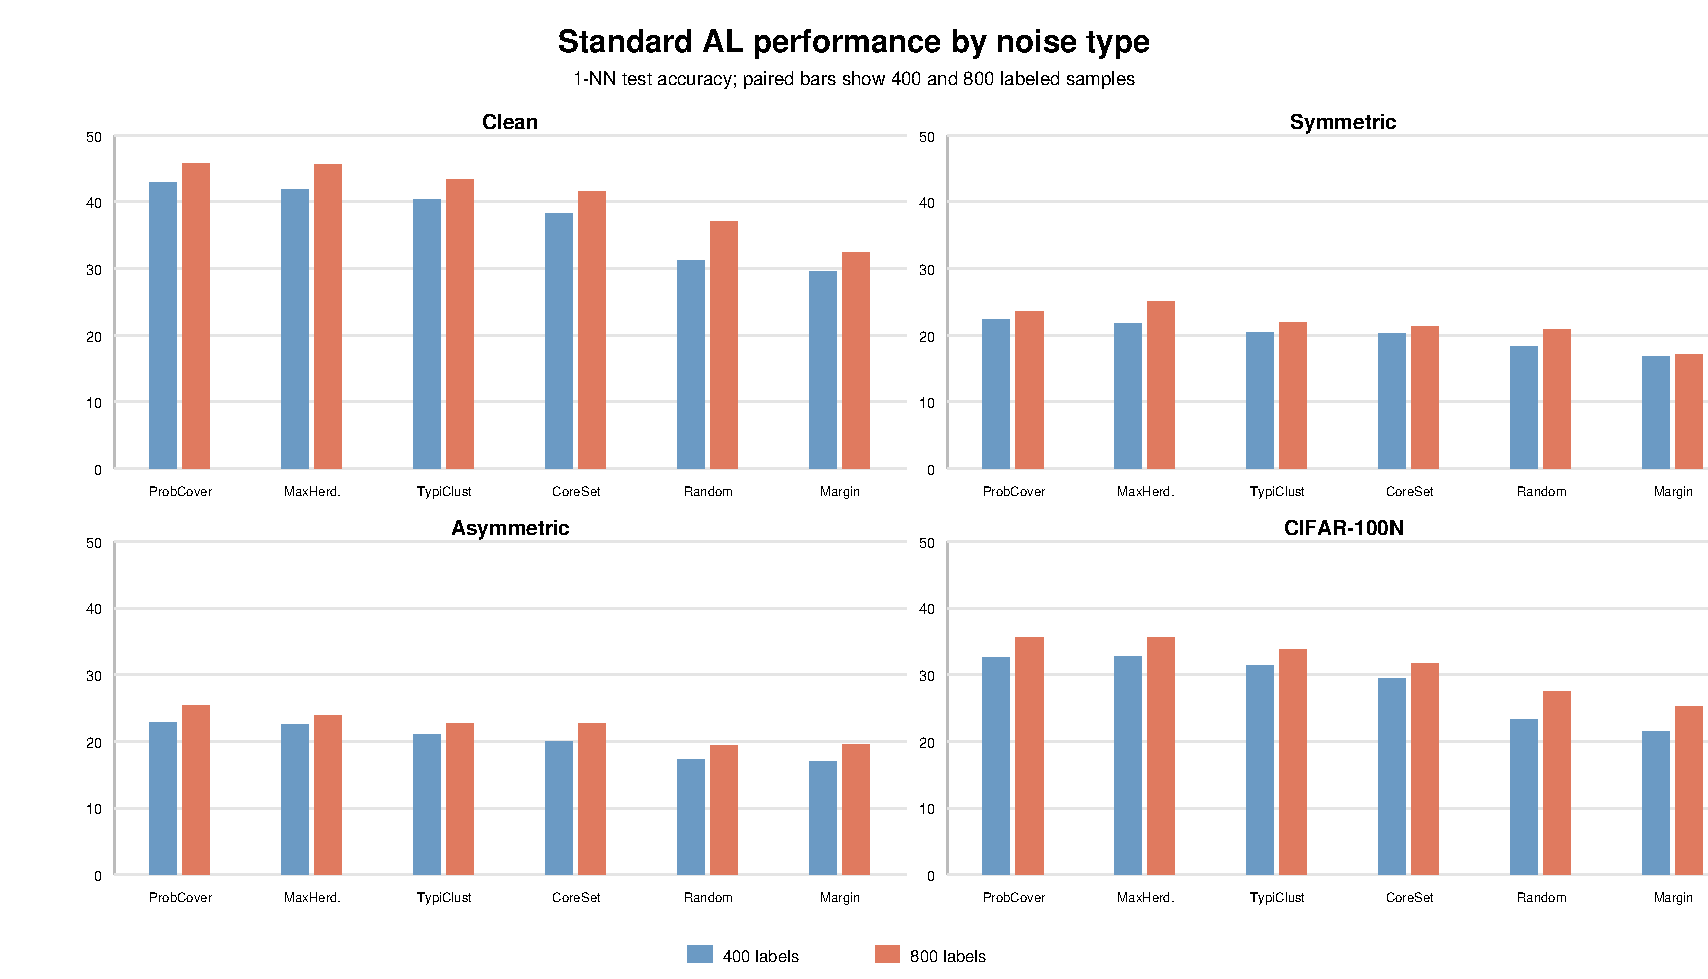
\includegraphics[width=0.96\textwidth]{figures/standard_al_by_noise.pdf}
  \caption{Standard AL methods under four noise settings. The main pattern is
  stable, but the small difference between \pc{} and \mh{} changes sign across
  noise types. Results use one seed and should not be read as uncertainty
  estimates.}
  \label{fig:standard}
\end{figure*}

\begin{table}[t]
  \centering
  \caption{Standard 1-NN test accuracy (\%). Means are over the four noise
  settings; the last columns show why per-noise comparisons matter.}
  \label{tab:standard}
  \resizebox{\columnwidth}{!}{\begin{tabular}{lrrrr}
\toprule
Method & Mean 400 & Mean 800 & Sym. 800 & Asym. 800 \\
\midrule
ProbCover & 30.17 & 32.60 & 23.56 & 25.45 \\
MaxHerding & 29.75 & 32.55 & 25.10 & 23.89 \\
TypiClust & 28.28 & 30.44 & 21.95 & 22.63 \\
CoreSet & 26.98 & 29.30 & 21.25 & 22.65 \\
Random & 22.52 & 26.16 & 20.80 & 19.38 \\
Margin & 21.23 & 23.58 & 17.14 & 19.51 \\
\bottomrule
\end{tabular}
}
\end{table}

\subsection{Direct cleaning changes labels, not performance}

Table~\ref{tab:cleaning} compares each cleaner with the matched CE run at 800
labels over 24 AL/noise settings. Checkpoint cleaning and direct AUM perform the
same 551 label-change operations in these runs. Only 238 changes correct a
wrong label, while 174 turn a known clean label into a wrong one. Their average
1-NN gain is only 0.23 points and the linear score changes by $-0.01$.
Temporal cleaning is slightly more conservative but leads to the same conclusion.
Cross-validation changes only one label across the whole grid, which makes it
safe but practically inactive.

The 1-NN metric can increase slightly because it uses the stored labels of the
selected neighbors. The linear classifier does not receive a meaningful
benefit, showing that the positive 1-NN delta should not be interpreted as a
general improvement. At this budget, a confident wrong prediction can easily
corrupt a clean example because many classes have very few labeled samples.

\begin{table*}[t]
  \centering
  \caption{Direct cleaning at 800 labels, averaged over matched settings.
  Change counts are totals over 24 runs and AL episodes, not unique images.}
  \label{tab:cleaning}
  \begin{tabular}{lrrrrr}
\toprule
Method & $\Delta$1-NN & $\Delta$linear & Changes & Correct & Clean$\to$wrong \\
\midrule
Checkpoint & +0.23 & -0.01 & 551 & 238 & 174 \\
Cross-validation & +0.00 & +0.00 & 1 & 1 & 0 \\
Temporal & +0.17 & -0.02 & 438 & 192 & 138 \\
AUM & +0.23 & -0.01 & 551 & 238 & 174 \\
\bottomrule
\end{tabular}

\end{table*}

\subsection{Robust losses: GCE underfits}

Losses are compared on the linear classifier. Margin is excluded from the
matched average because changing its loss also changes its acquisition scores
and selected set. For the five label-independent selectors, the image subset
and 1-NN result are unchanged across losses.

Bootstrap-soft remains very close to CE: its mean change is $+0.10$ at 400 labels
and $+0.22$ at 800. Bootstrap-hard is slightly worse. In contrast, \gce{}
loses \GCEFourDelta{} points at 400 labels and \GCEEightDelta{} at 800. The
result does not mean that robust losses are always harmful; instead, $q=0.7$ appears too
aggressive for a frozen linear model trained from very few samples. Early in
training, difficult clean examples also have small $p_y$, so \gce{} removes
useful learning signal together with noisy signal.

\begin{figure}[t]
  \centering
  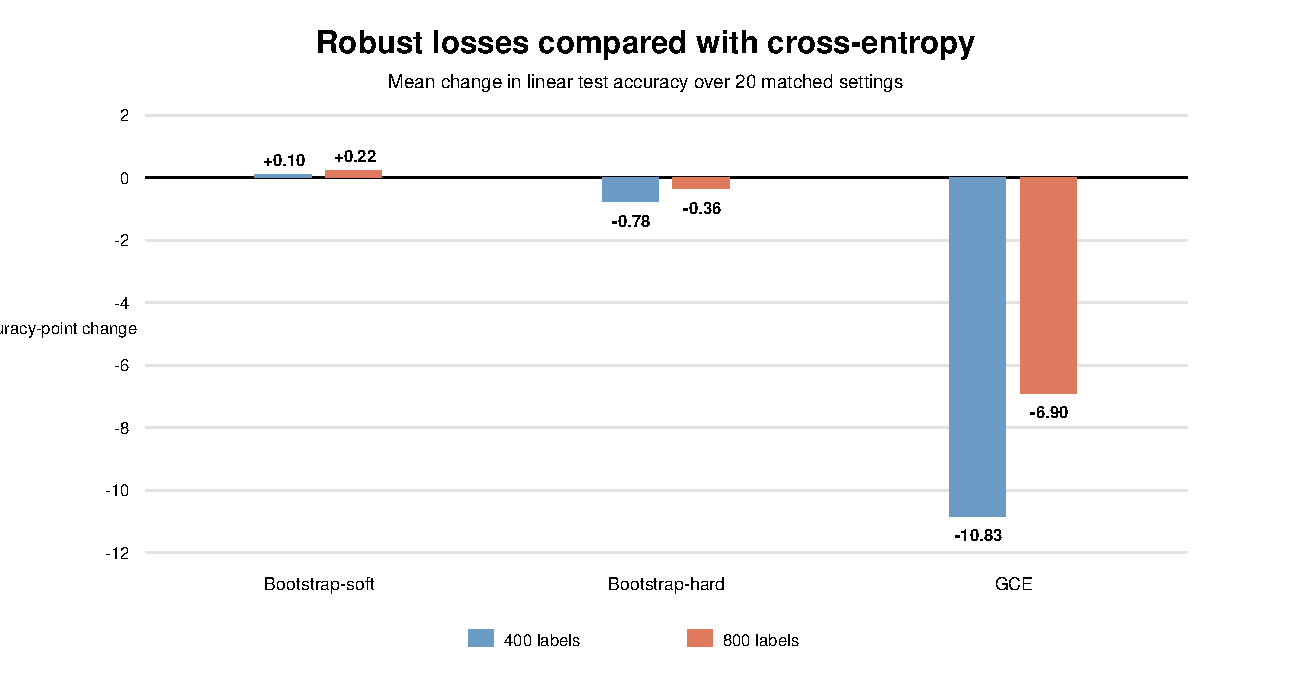
\includegraphics[width=\columnwidth]{figures/robust_loss_deltas.pdf}
  \caption{Mean linear-test change from cross-entropy over 20 matched settings
  per budget. GCE is clearly harmful with the tested hyperparameters.}
  \label{fig:losses}
\end{figure}

\begin{table}[t]
  \centering
  \caption{Robust-loss results (accuracy points). ``Linear, 800'' is the
  absolute mean test score.}
  \label{tab:losses}
  \resizebox{\columnwidth}{!}{\begin{tabular}{lrrr}
\toprule
Loss & $\Delta$ linear, 400 & $\Delta$ linear, 800 & Linear, 800 \\
\midrule
Bootstrap-soft & +0.10 & +0.22 & 31.22 \\
Bootstrap-hard & -0.78 & -0.36 & 30.64 \\
GCE & -10.83 & -6.90 & 24.11 \\
\bottomrule
\end{tabular}
}
\end{table}

\subsection{NPC depends on the selector and noise type}

\begin{figure*}[t]
  \centering
  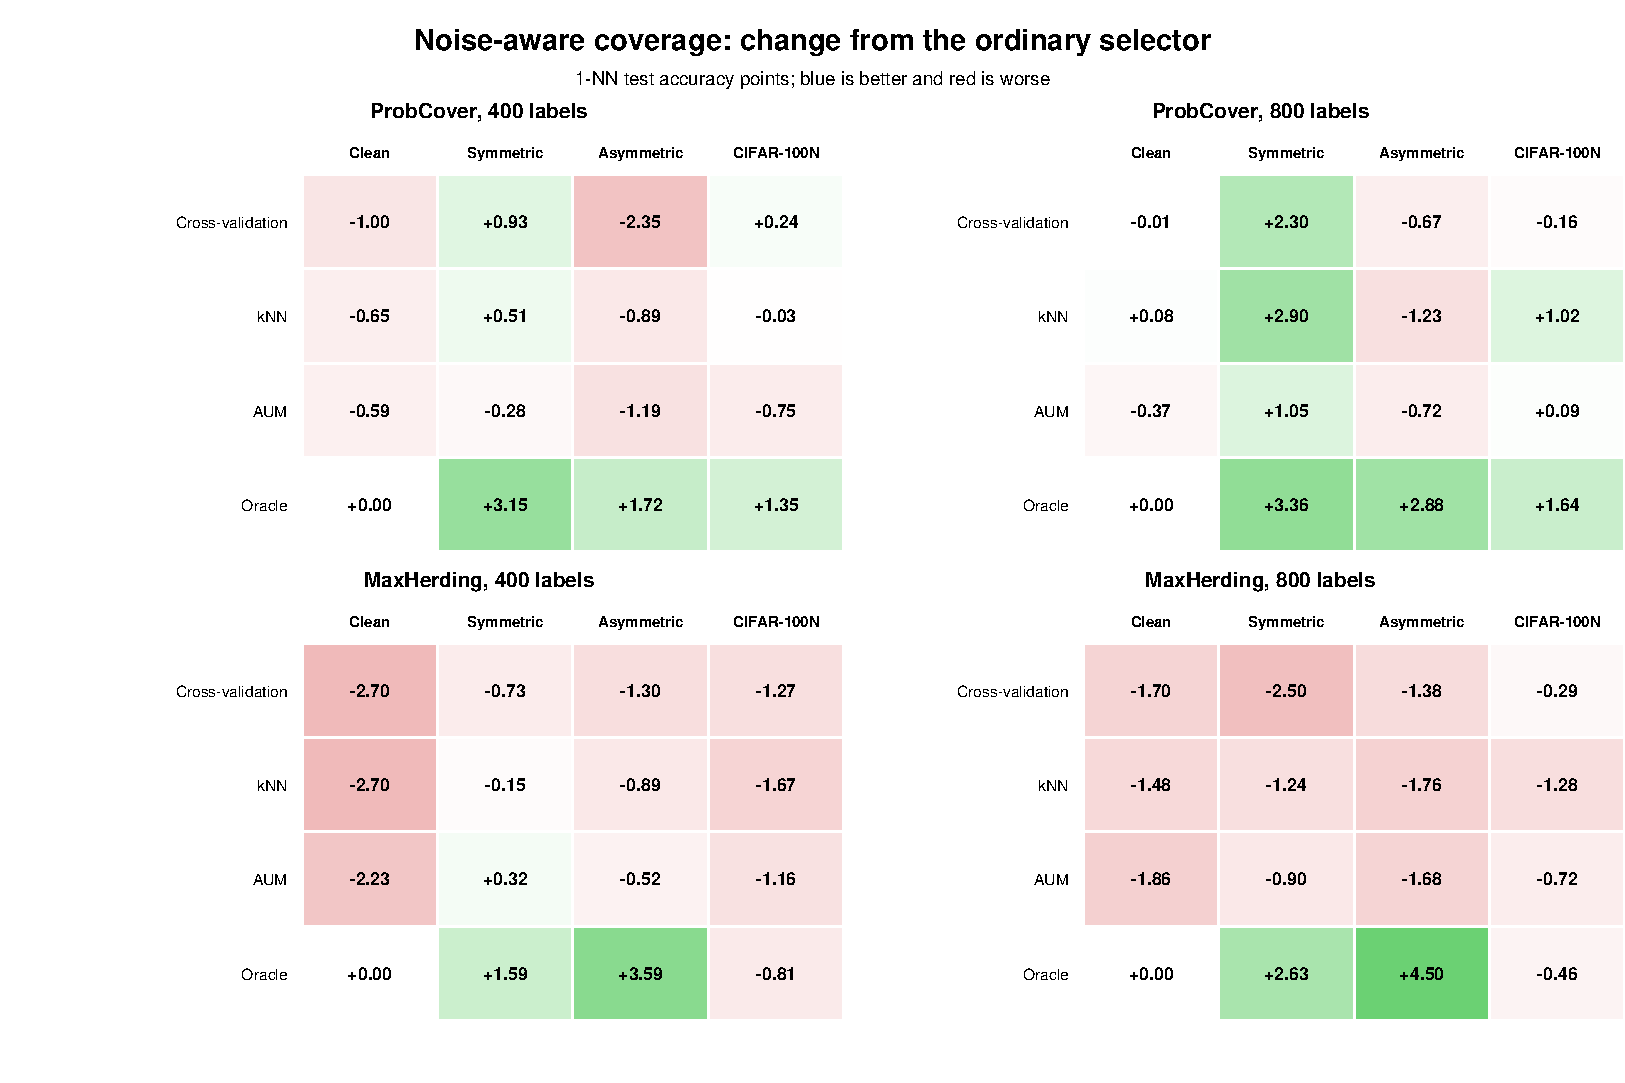
\includegraphics[width=0.90\textwidth]{figures/npc_deltas_by_noise.pdf}
  \caption{Change in 1-NN test accuracy from ordinary \pc{} or \mh{}. The new
  800-label \npc{-\pc{}} grid reveals useful symmetric-noise gains, while the
  same practical detectors remain harmful for \mh{} on average.}
  \label{fig:npc}
  \vspace{0.5em}
  \begin{minipage}{0.92\textwidth}
    \centering
    \captionof{table}{Mean NPC change from the matching ordinary selector,
    averaged over the four noise settings (1-NN accuracy points).}
    \label{tab:npc}
    \begin{tabular}{llrrrr}
\toprule
Selector & Budget & Cross-val & kNN & AUM & Oracle \\
\midrule
ProbCover & 400 & -0.55 & -0.27 & -0.70 & +1.56 \\
ProbCover & 800 & +0.36 & +0.69 & +0.01 & +1.97 \\
MaxHerding & 400 & -1.50 & -1.35 & -0.90 & +1.09 \\
MaxHerding & 800 & -1.47 & -1.44 & -1.29 & +1.67 \\
\bottomrule
\end{tabular}

  \end{minipage}
\end{figure*}

The 800-label \npc{-\pc{}} results substantially update the conclusion of the older report.
On symmetric noise, kNN improves 1-NN by \PCSymKNNDelta{} points,
cross-validation by \PCSymCVDelta{}, and AUM by \PCSymAUMDelta{}. kNN also
improves CIFAR-100N by 1.02 points. Averaged over all four noise settings, the
practical 800-label \npc{-\pc{}} deltas are $+0.69$ for kNN, $+0.36$ for
cross-validation, and $+0.01$ for AUM. These are modest gains, but they show
that a practical detector can help once the labeled set is large enough.

However, this pattern is not universal. At 400 labels all three practical \npc{-\pc{}}
averages are negative. On asymmetric noise at 800, they are also negative even
though the oracle improves by 2.88 points. This means the coverage idea can
help, but the practical detector still confuses hard clean points with noisy
ones. Clean-label runs are another useful check: the detector should ideally
remove nothing, yet practical filtering sometimes lowers accuracy.

For \npc{-\mh{}}, every practical detector is negative on average at both
budgets. The 800-label mean changes range from $-1.29$ to $-1.47$ points.
Meanwhile, the oracle gains 1.67 points on average, mainly because it improves
symmetric and asymmetric noise. The oracle is slightly worse on CIFAR-100N,
which also shows that perfect identification of wrong labels does not guarantee
that removing their coverage is optimal for every noise distribution.

\section{Conclusions and limitations}

The clearest positive result is the strength of representation-space coverage:
\pc{} and \mh{} select better labeled sets than Random, Margin, and CoreSet in
this low-budget experiment. Their relative order depends on the noise type, so
one averaged ranking is not enough. The strongest negative result is \gce{},
which underfits badly with the copied $q=0.7$ setting. Bootstrap losses are much
closer to CE and direct relabeling does not improve the trained linear model.

Noise-aware coverage is the most promising, but also the least consistent, part.
The completed 800-label grid shows that practical \npc{-\pc{}} can help under
symmetric noise. However, applying the same detector to \mh{} usually hurts,
and asymmetric noise remains difficult. My main conclusion is therefore not
that one detector ``solves'' noisy AL. It is that the interaction between the
coverage kernel and the detector matters, and detectors need enough labeled
examples before their decisions become useful.

There are important limitations. All runs use one seed, so small gaps may be caused
by one initial set or query sequence. No standard deviation can be estimated.
The representation is frozen, and robust losses may behave differently when a
deep network is fine-tuned and can memorize noise. The AUM implementation was
adapted for the low-budget setting and still does not exactly match the
reference implementation. Finally, the CSV summarizes final outcomes but does
not contain the detailed detector confusion counts for every newly completed
run, so I do not report updated precision or recall values.

The next experiment should repeat a smaller, focused grid over several seeds:
ordinary \pc{}/\mh{}, kNN-NPC, cross-validation-NPC, and the oracle under
symmetric and asymmetric noise. It would also be useful to delay filtering
until each class has several labeled neighbors and to tune \gce{} specifically
for the frozen linear classifier instead of reusing deep-network defaults.

\begin{thebibliography}{9}\small

\bibitem{shafir2025noisy}
N. Shafir, G. Hacohen, and D. Weinshall.
\newblock Active Learning with a Noisy Annotator.
\newblock \emph{arXiv preprint arXiv:2504.04506}, 2025.

\bibitem{hacohen2022typiclust}
G. Hacohen, A. Dekel, and D. Weinshall.
\newblock Active Learning on a Budget: Opposite Strategies Suit High and Low Budgets.
\newblock \emph{ICML}, 2022.

\bibitem{yehuda2022probcover}
O. Yehuda, A. Dekel, G. Hacohen, and D. Weinshall.
\newblock Active Learning Through a Covering Lens.
\newblock \emph{NeurIPS}, 2022.

\bibitem{bae2024maxherding}
W. Bae, J. Noh, and D. J. Sutherland.
\newblock Generalized Coverage for More Robust Low-Budget Active Learning.
\newblock \emph{ECCV}, 2024.

\bibitem{sener2018coreset}
O. Sener and S. Savarese.
\newblock Active Learning for Convolutional Neural Networks: A Core-Set Approach.
\newblock \emph{ICLR}, 2018.

\bibitem{wei2022cifarn}
J. Wei, Z. Zhu, H. Cheng, T. Liu, G. Niu, and Y. Liu.
\newblock Learning with Noisy Labels Revisited: A Study Using Real-World Human Annotations.
\newblock \emph{ICLR}, 2022.

\bibitem{pleiss2020aum}
G. Pleiss, T. Zhang, E. Elenberg, and K. Q. Weinberger.
\newblock Identifying Mislabeled Data using the Area Under the Margin Ranking.
\newblock \emph{NeurIPS}, 2020.

\bibitem{zhang2018gce}
Z. Zhang and M. Sabuncu.
\newblock Generalized Cross Entropy Loss for Training Deep Neural Networks with Noisy Labels.
\newblock \emph{NeurIPS}, 2018.

\bibitem{reed2015bootstrapping}
S. Reed, H. Lee, D. Anguelov, C. Szegedy, D. Erhan, and A. Rabinovich.
\newblock Training Deep Neural Networks on Noisy Labels with Bootstrapping.
\newblock \emph{ICLR Workshop}, 2015.

\end{thebibliography}

\end{document}
